\chapter{SYSTEM OVERVIEW}\label{chapter_system_overview}
%\pagebreak
The Top level handwriting recognition system is divided into four sub-systems, image acquisition, preprocessing, feature extraction and recognition. The top level model of proposed system is given in Figure \ref{figure_system_overview}.
\begin{figure}[h]
\centering
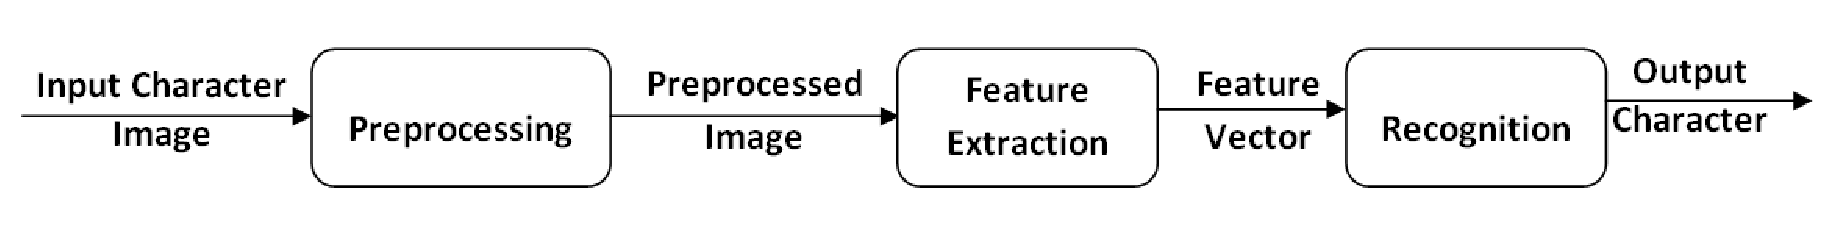
\includegraphics[width=\linewidth]{figures/system_overview/system_overview.eps}
\caption{Off-line Handwriting Recognition System.}
\label{figure_system_overview}
\end{figure}

The basic system architecture of the image acquisition, preprocessing, feature extraction and recognition is briefly described in section \ref{section_image_acquisition}, section \ref{section_image_preprocessing}, section \ref{section_feature_extraction} and section \ref{section_recognition}, respectively.

\section{Image Acquisition} \label{section_image_acquisition}
Images are acquired by scanning the handwritten documents using digital scanners or by taking photograph of the handwriting document using digital camera. CANON LIDE scanner is used to scan the handwritten samples from different writers. Each images are scanned at 300dpi in RGB color mode. Detail of the handwritten corpus used for the experimentation is given in chapter \ref{chapter_nepali_handwritten_database}. Figure \ref{figure_image_slicing} shows the slicing of off-line character images from handwritten samples and Figure \ref{figure_image_acquisition} shows the final stage of the image acquisition.

\begin{figure}[h]
\centering
\begin{tabular}{cc}
\includegraphics[scale=0.70]{figures/system_overview/image_acquisition.eps} & \includegraphics[scale=0.70]{figures/system_overview/image_slicing1.eps}
\end{tabular}
\caption{Image Slicing.}
\label{figure_image_slicing}
\end{figure}
\pagebreak
\begin{figure}[h]
\centering
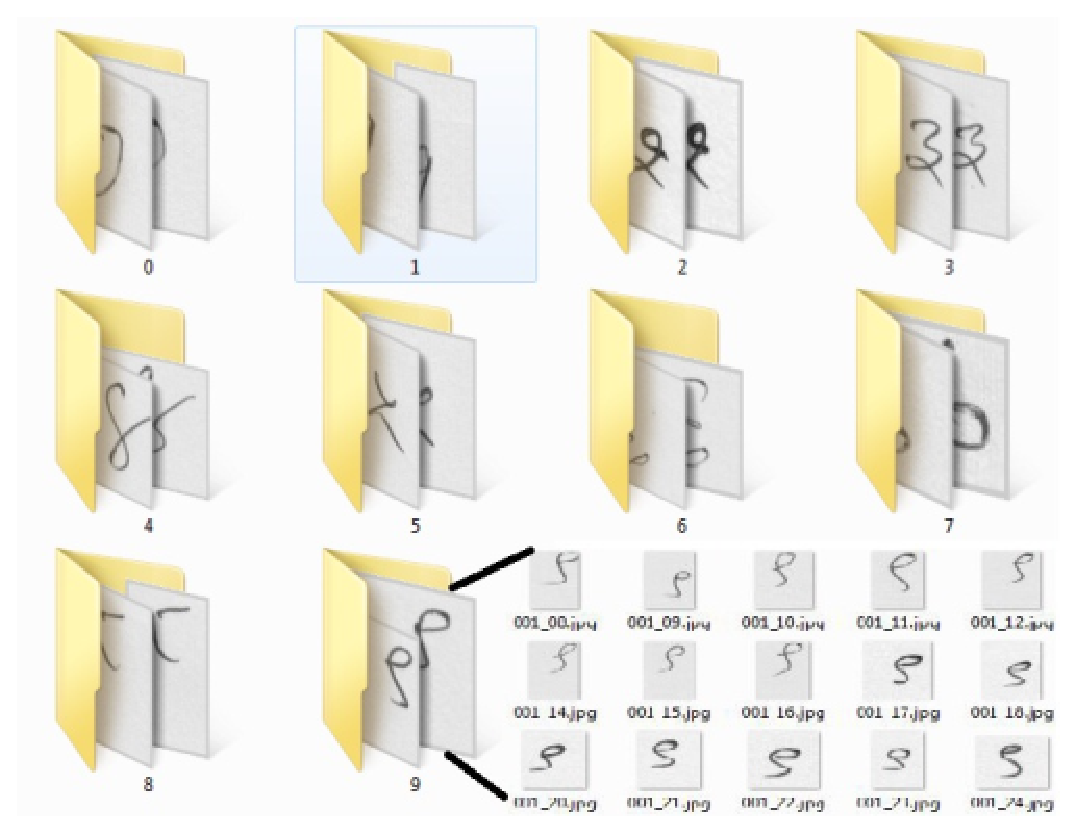
\includegraphics[scale=0.5]{figures/system_overview/folders_files.eps}
\caption{Image Acquisition.}
\label{figure_image_acquisition}
\end{figure}

\newpage
\section{Image Preprocessing} \label{section_image_preprocessing}
Pre-processing is done prior to feature extraction algorithms. The raw images are subjected to a number of preliminary processing steps to make it usable in the descriptive stages of character analysis. Pre-processing aims to produce clean document images that are easy for the Recognition systems to operate accurately. The block diagram of preprocessing system is given in Figure \ref{figure_image_preprocessing}. Details of the each preprocessing steps is described in the section \ref{section_preprocessing_methodology}.
\begin{figure}[h]
\centering
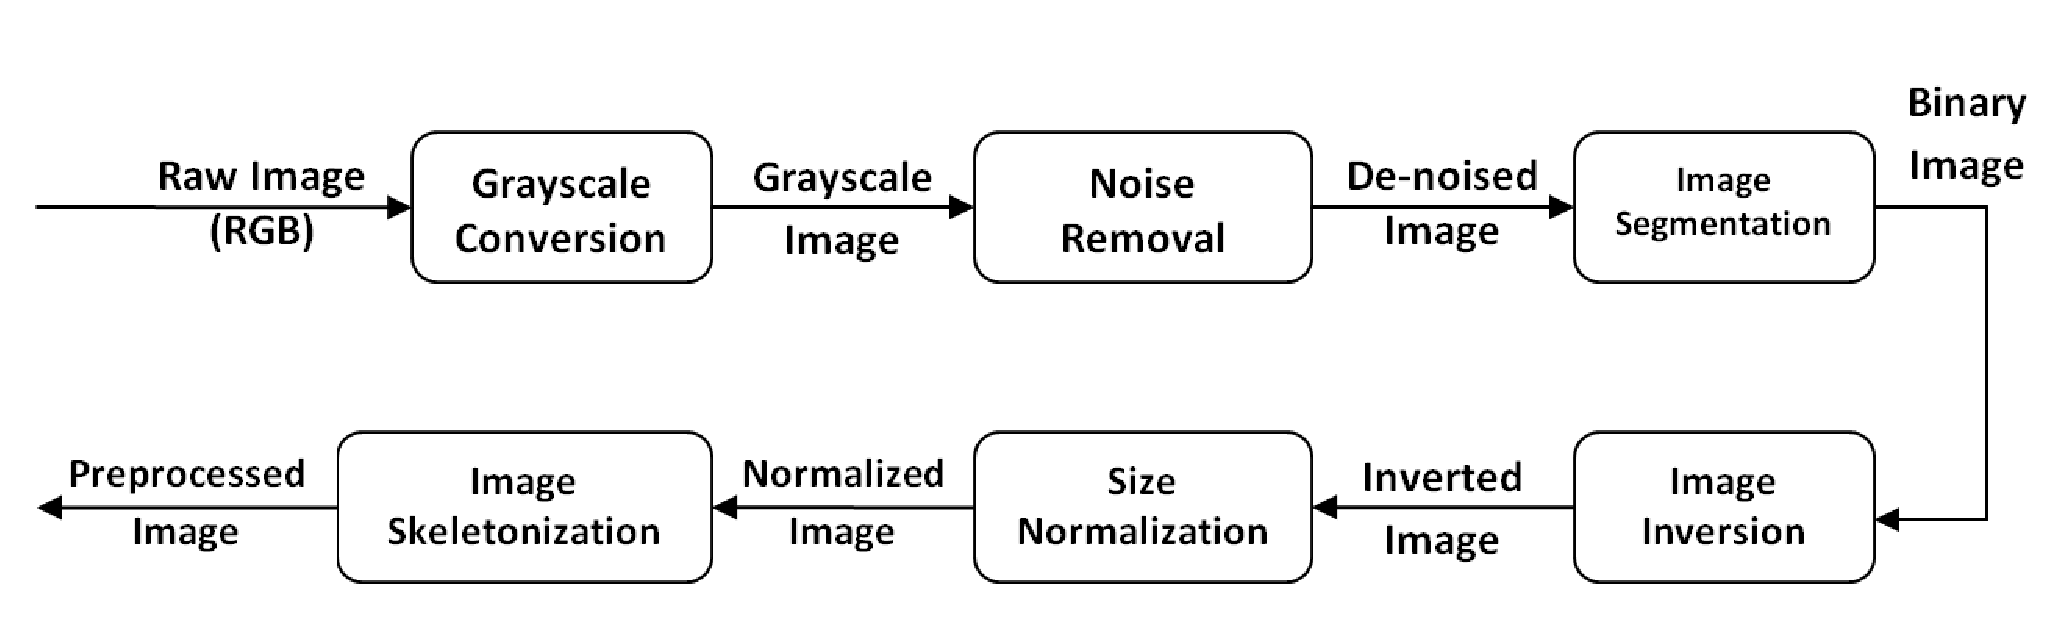
\includegraphics[width=\linewidth]{figures/system_overview/image_preprocessing.eps}
\caption{Image Preprocessing.}
\label{figure_image_preprocessing}
\end{figure}


\section{Feature Extraction} \label{section_feature_extraction}
After pre-processing of the character images, feature vectors are extracted, which is used in the training and recognition stage. Feature sets play one of the most important roles in a recognition system. A good feature set should represent characteristic of a class that helps distinguish it from other classes, while remaining invariant to characteristic differences within the class. The high level block diagram of the feature extraction system is given in the Figure \ref{figure_feature_extraction}. Detail description of each feature extraction techniques is given in section \ref{section_feature_extraction_methodology}.
\begin{figure}[h]
\centering
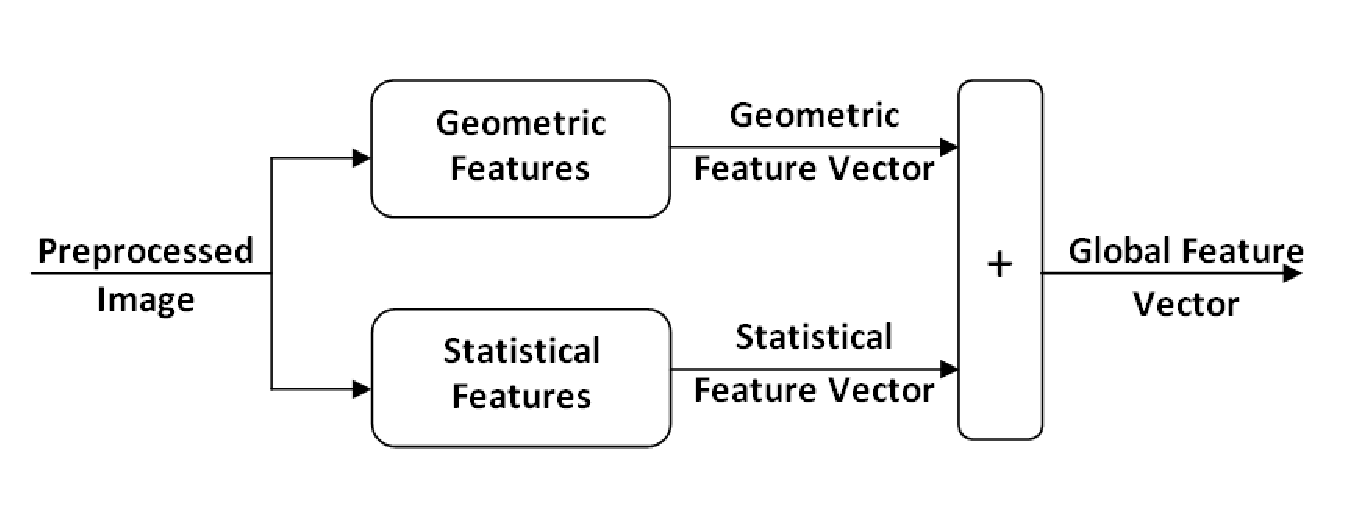
\includegraphics[width=5in]{figures/system_overview/feature_extraction.eps}
\caption{Feature Extraction.}
\label{figure_feature_extraction}
\end{figure}

\pagebreak
\section{Recognition} \label{section_recognition}
Recognition engine of the system consists of two neural network based algorithms implemented in it. There are two stages of the recognition, training and testing. In the training stage system learns how to behave in the new environment of similar inputs and in the testing stage accuracy of the classification is determined. The top level recognition system is given in figure \ref{figure_recognition}. Detail of the each algorithms used in the recognition system is given in the section \ref{section_training_testing_methodology}.


\begin{figure}[h]
\centering
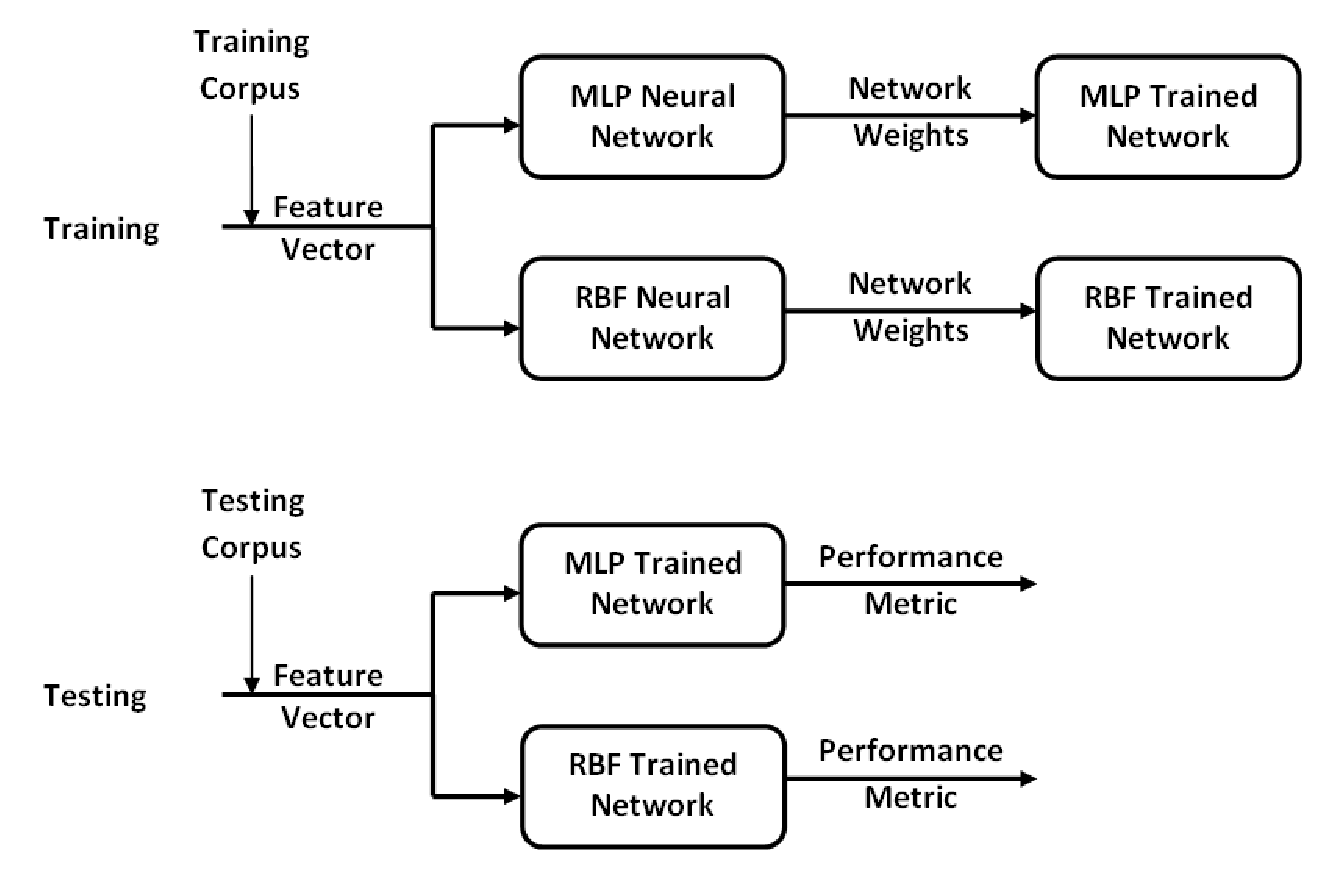
\includegraphics[width=4.50in]{figures/system_overview/testing_training.eps}
\caption{Training and Testing.}
\label{figure_recognition}
\end{figure}
